
\chapter{Modal Logic}
\dfn{Language}
{The language or modal logic consists of:
        \begin{itemize}
                \item Propositional variables: $p_1,p_2,p_3,\cdots$ where $i \in \{0\}\cup \mathbb{N}$ but often, these are going to be just lowercase letter.
                \item Connectives:
                        \begin{itemize}
                                \item $\wedge$ - conjunction
                                \item  $\vee$ - discjnction 
                                \item $\rightarrow$ - implication
                                \item $\leftrightarrow$ - equivalence
                                \item  $\neg$ - negation
                                \item $\Box$ - (colloguialy) always
                                \item  $\Diamond$ (calloguialy) sometimes
                        \end{itemize}
                 \item brackets - (,)
                 \item (sometimes) Two constants : $\mathbb{1},\mathbb{0}$


        \end{itemize}        
}

\dfn{Sentences}
{
 The set of sentences is the smallest set of words(over a desribed alphabet) $\mathcal{S}$ satisfying the following propperties:
        \begin{itemize}
                \item $\forall n \in \mathbb{N} \: p_n \in \mathcal{S}$ 
                \item if $\phi, \psi \in \mathcal{S}$ then $(\phi \wedge \psi)$, $\phi \vee \psi$, $\cdots$,$\Box \phi \in \mathcal{S}$ 
        \end{itemize}
}

\dfn{Kripke's frame}
{
        A krpkes frame is a pair (X,R), where X is a set and R is a relation on X, ie. $R \subset X \times X$
 \ex{(X,R)}
  {
          A simple example of a Kripke's frame can be visualised for given sets X and R using a directed graph, where the nodes are elements of X, and edges elements of R. The given sets are:
          \begin{itemize}
                  \item $X = \{a,b,c,d\}$
                  \item  $R = \{(a,a),(a,b),(b,c),(c,b),(c,d),(d,d)\}$
          \end{itemize}
          \begin{center}
                  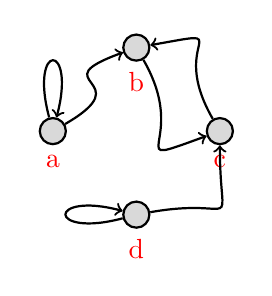
\begin{tikzpicture}[thick,node distance = {15mm},  main/.style = {draw, circle}, loop/.style={min distance = 10mm, looseness=10}]
                  \node[main, fill = gray!30, label={[red]below:a}](1) {};
                  \node[main, fill = gray!30, label={[red]below:b}](2)[above right of=1] {};
                  \node[main, fill = gray!30, label={[red]below:c}](3)[below right of =2] {};
                  \node[main, fill = gray!30, label={[red]below:d}](4)[below left of=3] {};
                  \draw[->] (1) to [loop above] (1);
                  \draw[->] (1) to [out=30, in=200, looseness=2.5] (2);
                  \draw[->] (2) to [out=300, in=200, looseness=2.5] (3);
                  \draw[->] (3) to [out=120, in=10, looseness=2.5] (2);
                  \draw[->] (4) to [out=10, in=270, looseness=2.5] (3);
                  \draw[->] (4) to [loop left] (4);
                  
          \end{tikzpicture}
          \end{center}
  }
}
\dfn{Kripke's model}
{
        A Kripke's model is a triple $(X,R,\pi) = \mathbb{M}$, where (X,R) is a Kripke's frame.
        $\pi$ is a function $\pi \,:\,\mathcal{P} \longrightarrow P(x) $, where $P(x)$ is a valuation.

 \ex{(X,R,$\pi$)}
  {
          Krikpe's model will be visualised as Kripke's frame was before. What this means, is that p is true in a and b, but nowhere else
          \begin{center}
                  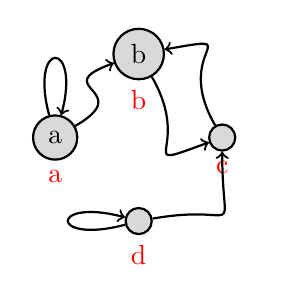
\begin{tikzpicture}[thick,node distance = {15mm},  main/.style = {draw, circle}, loop/.style={min distance = 10mm, looseness=10}]
                          \node[main, fill = gray!30, label={[red]below:a}](1) {{a}};
                          \node[main, fill = gray!30, label={[red]below:b}](2)[above right of=1] {{b}};
                  \node[main, fill = gray!30, label={[red]below:c}](3)[below right of =2] {};
                  \node[main, fill = gray!30, label={[red]below:d}](4)[below left of=3] {};
                  \draw[->] (1) to [loop above] (1);
                  \draw[->] (1) to [out=30, in=200, looseness=2.5] (2);
                  \draw[->] (2) to [out=300, in=200, looseness=2.5] (3);
                  \draw[->] (3) to [out=120, in=10, looseness=2.5] (2);
                  \draw[->] (4) to [out=10, in=270, looseness=2.5] (3);
                  \draw[->] (4) to [loop left] (4);
                  
          \end{tikzpicture}
          \end{center}
  }
}



\dfn{Modal theories}
{
    $T \subset \mathcal{L}_{ML}(\mathcal{P}) $ is a modal theory.
}
\dfn{T- tautology}
{
    $\phi \in \mathcal{L}_{ML}(P)$ is a T tautology if
    \begin{itemize}
            \item for every frame (X,R) satisfying $(X,R) \vDash T$ we have $(X,R) \vDash \phi$.
            
    \end{itemize}
    We write $ \vDash T \phi$
    $(X,R) \vDash T$ means that $\forall \psi \in T \: (X,R) \vDash \psi $
}

\ex{Modal theory}
{
    \begin{itemize}
            \item $K = \empty$
            \item  $S_4 = \{ p \rightarrow \Diamond p, \Diamond \Diamond p \rightarrow p \} $
            \item $S_5 = S_4 \cup \{ p \rightarrow \Box \Diamond p\} $ 
So, K is a theory of all frames, S_4 is a theory "of preorders", S_5 is a theory of "equivalence relations"



            
    \end{itemize}
%          \begin{center}
%                  \begin{tikzpicture}[thick,node distance = {15mm},  main/.style = {draw, circle}, loop/.style={min distance = 10mm, looseness=10}]
%                          \node[main, fill = gray!30, label={[red]below:a}](1) {{a}};
%                          \node[main, fill = gray!30, label={[red]below:}](2)[right of=1] {{}};
%                          \node[main, fill = gray!30, label={[red]below:}](3)[bottom right of=1] {{}};
%                          \draw[->] (1) to [out=0, in=180, looseness=2.5] (2);
%                          \draw[->] (1) to [loop] (1) ;
%                          \draw[->] (2) to [out=270, in=90, looseness=2.5] (3);
%                          \draw[->] (3) to [out=1 , in=1, looseness=2.5] (1);
%                          
%                          
%                          
%                  
%          \end{tikzpicture}
%          \end{center}
%
    \ex{Modal tautologies}
    {
        \begin{equation}
            \vDash S_4 \: \Diamond \Diamond p \leftrightarrow \Diamond p      
        \end{equation}

    }

    \begin{myproof}
        \begin{itemize}
                \item $ \vDash s_4 \Diamond \Diamond p \rightarrow \Diamond       $ 
                \item $ \vDash S_4 \: \phi \rightarrow \Diamond  \phi  $ 
                \item $ \rightarrow  S_4 \Diamond p \rightarrow \Diamond \Diamond p      $ 
                \item $ \rightarrow S_4 \Diamond p \leftrightarrow \Diamond \Diamond p      $
        \end{itemize}



    \end{myproof}

        \begin{equation}
             \vDash S_4 \Box \Box \leftrightarrow \Box p      
        \end{equation}

    \begin{myproof}
        \begin{itemize}
                \item $ \Box \Box p \equiv_K \neg \neg \Box \Box p \leftrightarrow \neg \Diamond \neg \Box p \leftrightarrow \neg \Diamond \Diamond \neg p \leftrightarrow \\
\neg \Box \neg p \leftrightarrow \neg \neg \Box p \leftrightarrow \Box p      
                    $
                
        \end{itemize}
    \end{myproof}



    \qs{jprdle nic ne dziala mac kurwa, cala sekcja jest przekleta}{Find all nonequivalent sentences in $S_4(S_5)$ made of one propositional variable p and connectors $\Diamond , \Box$}
}


\section{Linear Temporal Logic}
    (Idea: It is the modal logic for one frame, i.e. $(\mathbb{N},\leq)$)
    We treat $\mathbb{N}$ as discrete time. ($\{0\} \in \mathbb{N}$)

    \dfn{Syntax}
    {
        \begin{itemize}
            \item $\mathcal{L}_{LTL}(\mathcal{P})$ -- $\mathcal{P}$ is a setof propositional variables, and $\mathcal{L}_{LTL}$ the set of sentences.
           \item our alphabet consists of $\mathcal{P}$, and the alphabet of modal logic, as well as two new symbols: $\bigcirc, \mathcal{U}$
                
        \end{itemize}

        What are these new connectors?
        \begin{itemize}
            \item $\phi \in \mathcal{L}_{LTL}(\mathcal{P}) \rightarrow \bigcirc \phi \in \mathcal{L}_{LTL}(\mathcal{P})$ 
            \item $\phi, \psi \in \mathcal{L}_{LTL}(\mathcal{P}) \rightarrow \phi \mathcal{U} \psi \in \mathcal{L}_{LTL}(\mathcal{P})$
                
        \end{itemize}


    }

    \dfn{Model}
    {
        A model is a valuation, i.e.  $\pi \,:\,\mathbb{N} \longrightarrow P(\mathcal{P}) $

    }
    \nt
    {
        We let $\phi \in \mathcal{L}_{LTL}(\mathcal{P})$. $\pi$ is a model, $n \in \mathbb{N}$. We want to define $\pi, n \vDash \phi$

        \begin{itemize}
            \item if $\phi = p \in \mathcal{P} \text{, then:  } \pi, n \vDash \leftrightarrow p \in \pi(n)$
            \item if $ \phi = \psi_1 \vee \psi_2 \text{, then:  }  \pi,n \vDash \psi_1 \vee  ps_2 \leftrightarrow  \pi,n \vDash \psi_1 \vee \pi,n \vDash ps_2$
            \item if $ \phi = \Diamond \psi \text{, then:  } \pi,n \vDash \Diamond \psi \leftrightarrow \exists  m \ge n  \pi,m \vDash \psi $
            \item if $\phi = \Box \psi \text{, then:  } \pi,n \vDash \Box \psi \leftrightarrow \forall m \ge n\: \pi, m \vDash \psi $ 
            \item if $\phi = \bigcirc \psi \text{, then:  } \pi,n \vDash \bigcirc \psi \leftrightarrow  \pi, n+1 \vDash \psi$ 
            \item if $ \phi = \psi_1 \mathcal{U} \psi_2 \text{, then:  } \pi, n \vDash \psi_1 \mathcal{U} \psi_2 \leftrightarrow  (\exists m \ge n )(\pi,m \vDash  \psi_2 \wedge (\forall k )(n \le k < m \rightarrow  \pi, k \vDash \psi_1)$
        \end{itemize}
    }


    \dfn{LTL - Tautology}
    {
        Let $\phi \in \mathcal{L}_{LTL}(\mathcal{P})$. We say that $\phi$ is an LTL tautology if:
        \begin{equation}
             \vDash_{LTL} \phi \: \text{ if } \forall \pi \forall n \: \pi,m \vDash \phi
        \end{equation}
    }

    \ex{Example LTL Tautology}
    {
        \begin{equation}
            \vDash_{LTL} q \rightarrow p \mathcal{U} q
        \end{equation}
        \\

        \begin{myproof}
            Fix $\pi, n$. Assume that $\pi, n \vDash q$. Then:
            \begin{equation}
                ( \exists m \ge n ) (\pi,m \vDash q \wedge (\forall k)(n \le k < m \rightarrow \pi, k \vDash p) )
            \end{equation}
            meaning $\pi, n \vDash p \mathcal{U} q$
        \end{myproof}
    }

    \ex{Another example}
    {
        \begin{equation}
            \pi \,:\,\mathbb{N} \longrightarrow P(\mathcal{P})  \pi = (\pi_1,\pi_2,\cdots )
        \end{equation}
        \begin{myproof}
            Let $\pi' = (\{q\}, \emptyset, \emptyset ),\cdots $, Then $\pi \bigcirc \vDash p \mathcal{U} q$ and $\pi,\bigcirc \vDash \neg \Diamond p$
         
        \end{myproof}
        \begin{myproof}
            Let $\pi' = (\{q_1\},\cdots )$, Then for every n $\pi', m \vDash p \mathcal{U} q$ \\
            But $\pi',n \vDash  \neg \Diamond p$
            
                
        \end{myproof}
    }
    \nt{Standard order $\le$ is a reflexive and transitive relation on  $\mathbb{N}$, os every $S_4$ tautology is LTL - tautology}

    \mlenma{}{In LTL we can get rif of sumbols $\Box , \Diamond $ Why?\\
    \begin{itemize}
        \item $ \vDash_{LTL} \Diamond \phi  \leftrightarrow (p \vee \neg p) \mathcal{U} \phi$ 
        \item $ \vDash _{TLT} \Box \phi \leftrightarrow \neg \Diamond \neg \phi$
            
    \end{itemize}
    }

    \mlenma{}{$ \vDash_{LTL} \phi$ iff $\forall \pi \: \pi,\bigcirc \vDash \phi $}

    \dfn{S - shift}
    {
        $S(a_0,a_1,\cdots ) = (a_1,a_2,\cdots )$
    }
    
   \qs{}{Prove that $\pi, n \vDash \phi \leftrightarrow  S^n \pi, \bigcirc \vDash \phi$}

   \qs{}{What can be described using LTL?}
   \ex{LTL Descriptions}
   {
       \begin{itemize}
               \item $\Diamond \Box \alpha$ -- it means that $\alpha$ will be true from some point in tie on
               
               \item $\Box \Diamond \beta$ -- it means that $\beta$ will hapen  $\inf$--many times.
       \end{itemize}
   }




